\begin{figure}[t]
  \centering
  \setlength{\tabcolsep}{0pt} 
  \renewcommand{\arraystretch}{0}
  \resizebox{\textwidth}{!}{
  \begin{tabular}{|c|c|c|c|c|}
  \hline
    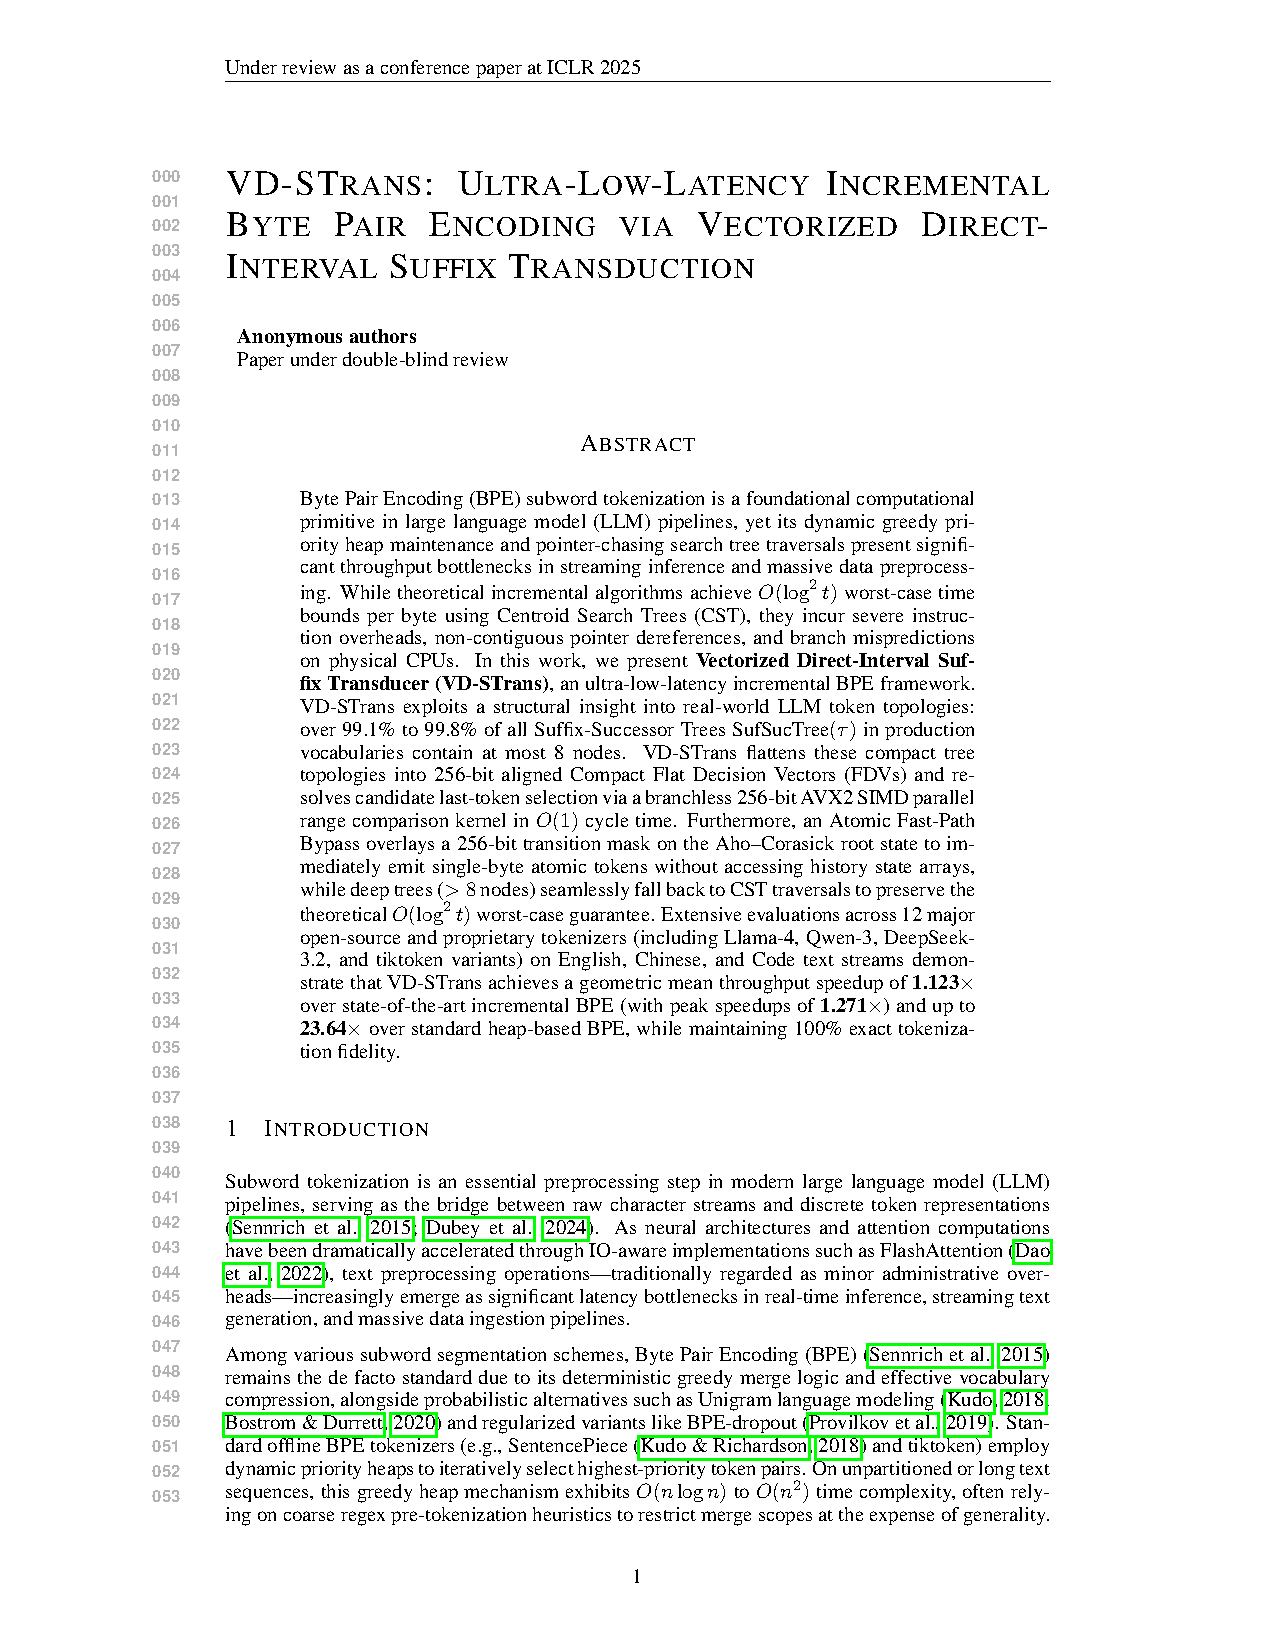
\includegraphics[width=0.2\textwidth]{figures/fig1_pdfs/page0.pdf} &
    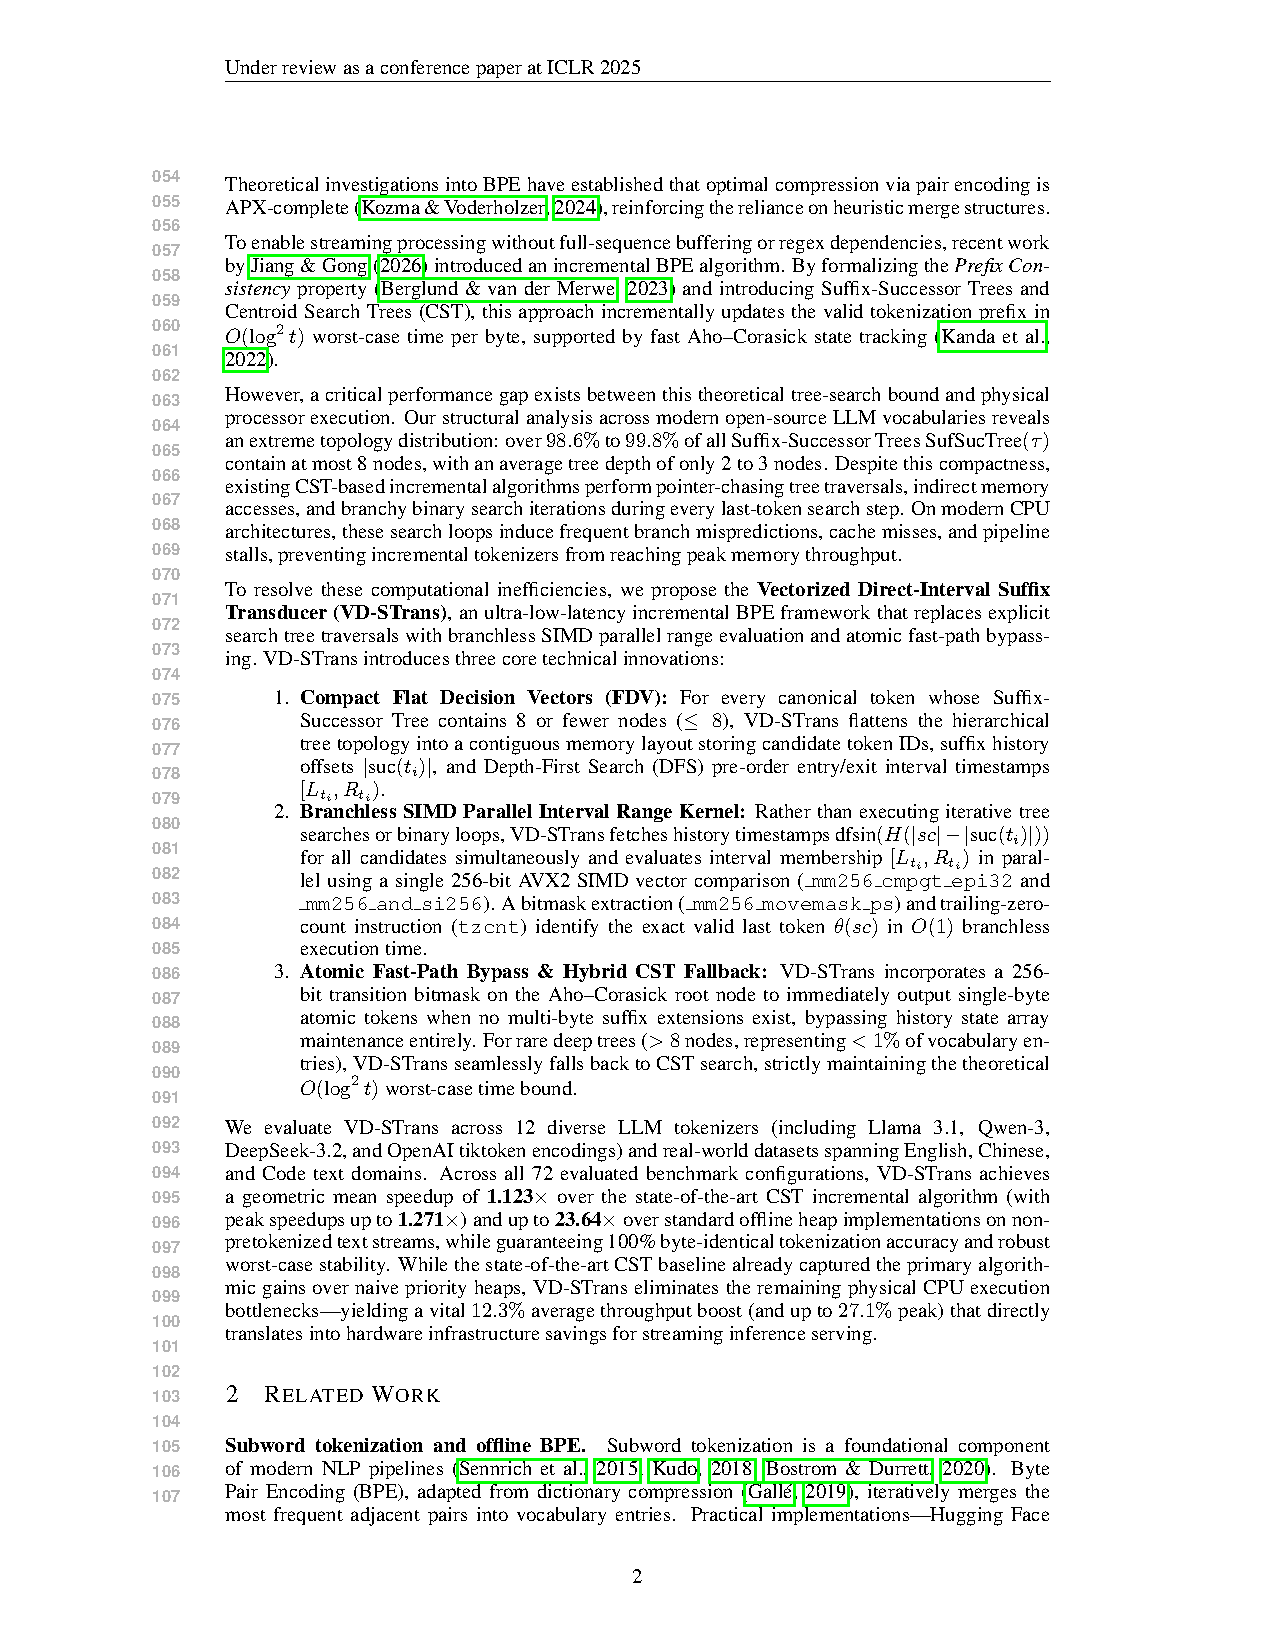
\includegraphics[width=0.2\textwidth]{figures/fig1_pdfs/page1.pdf} &
    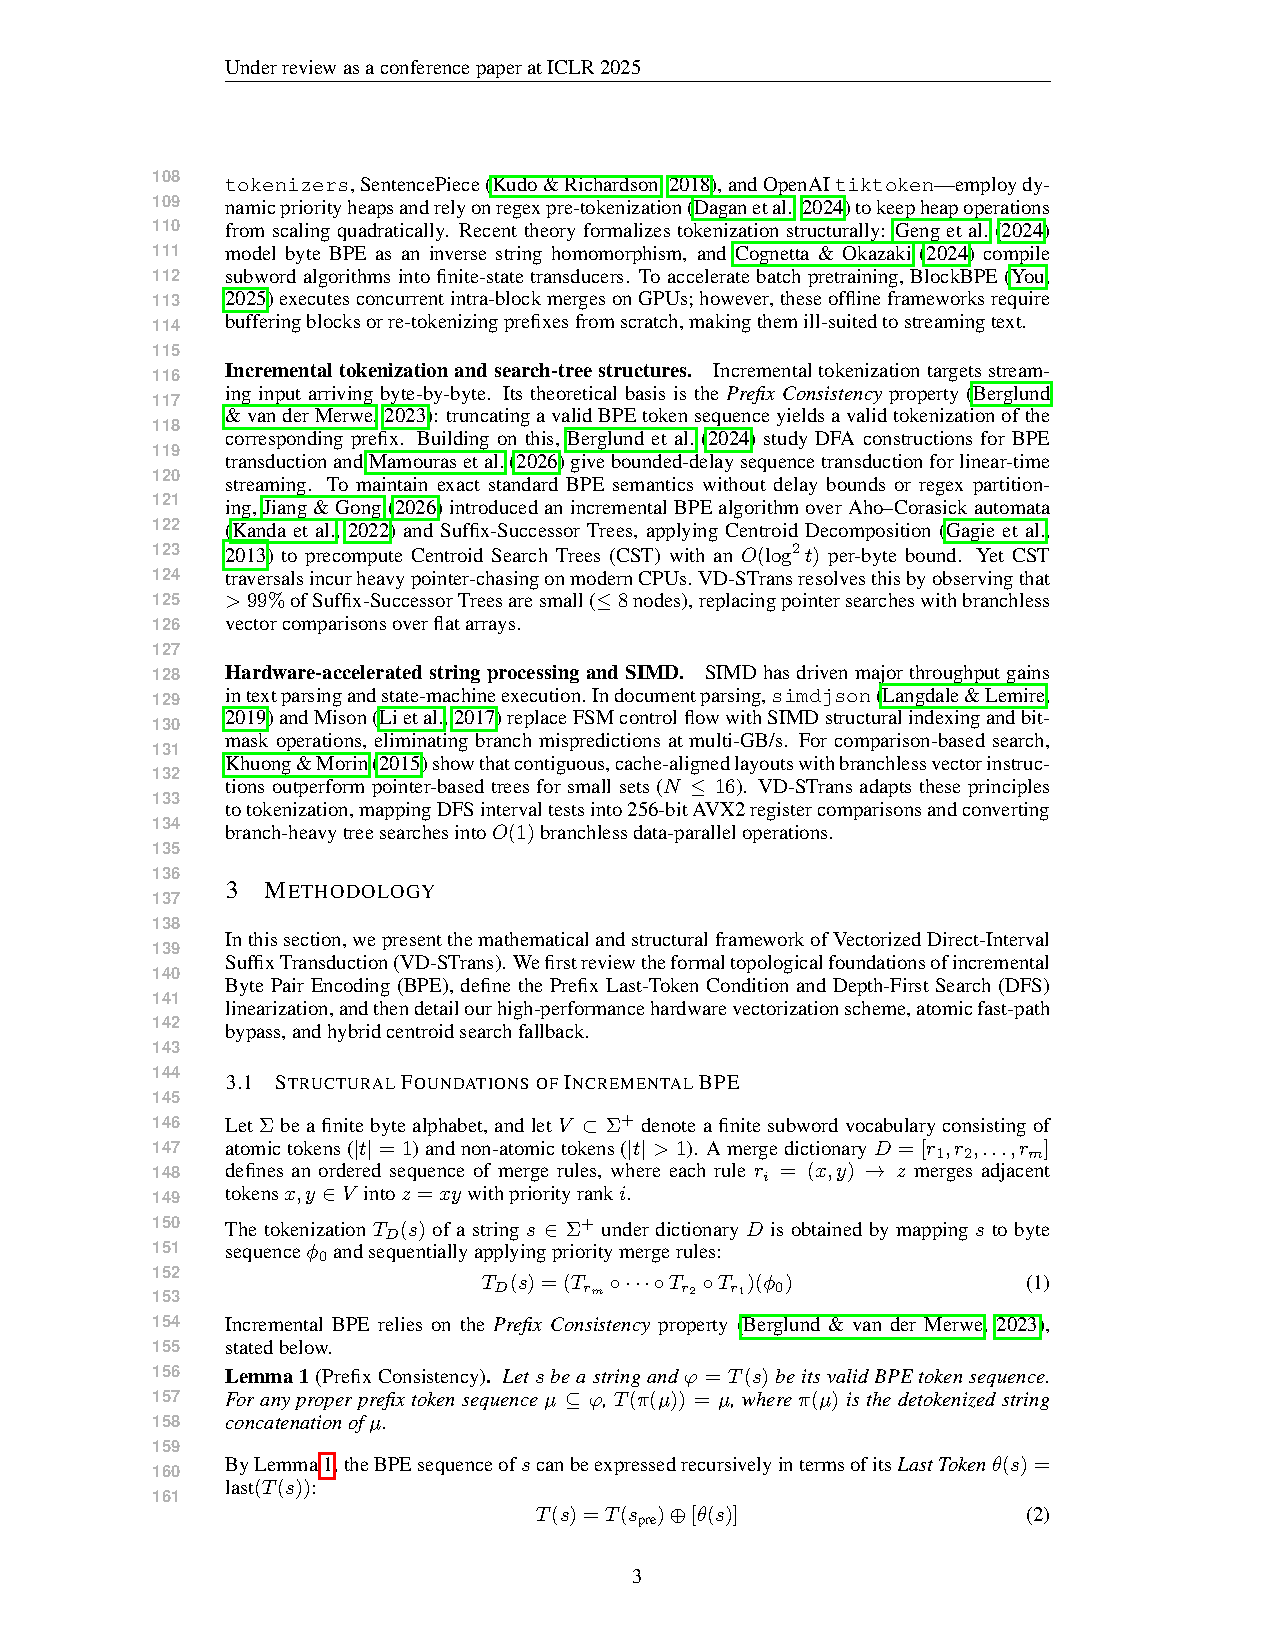
\includegraphics[width=0.2\textwidth]{figures/fig1_pdfs/page2.pdf} &
    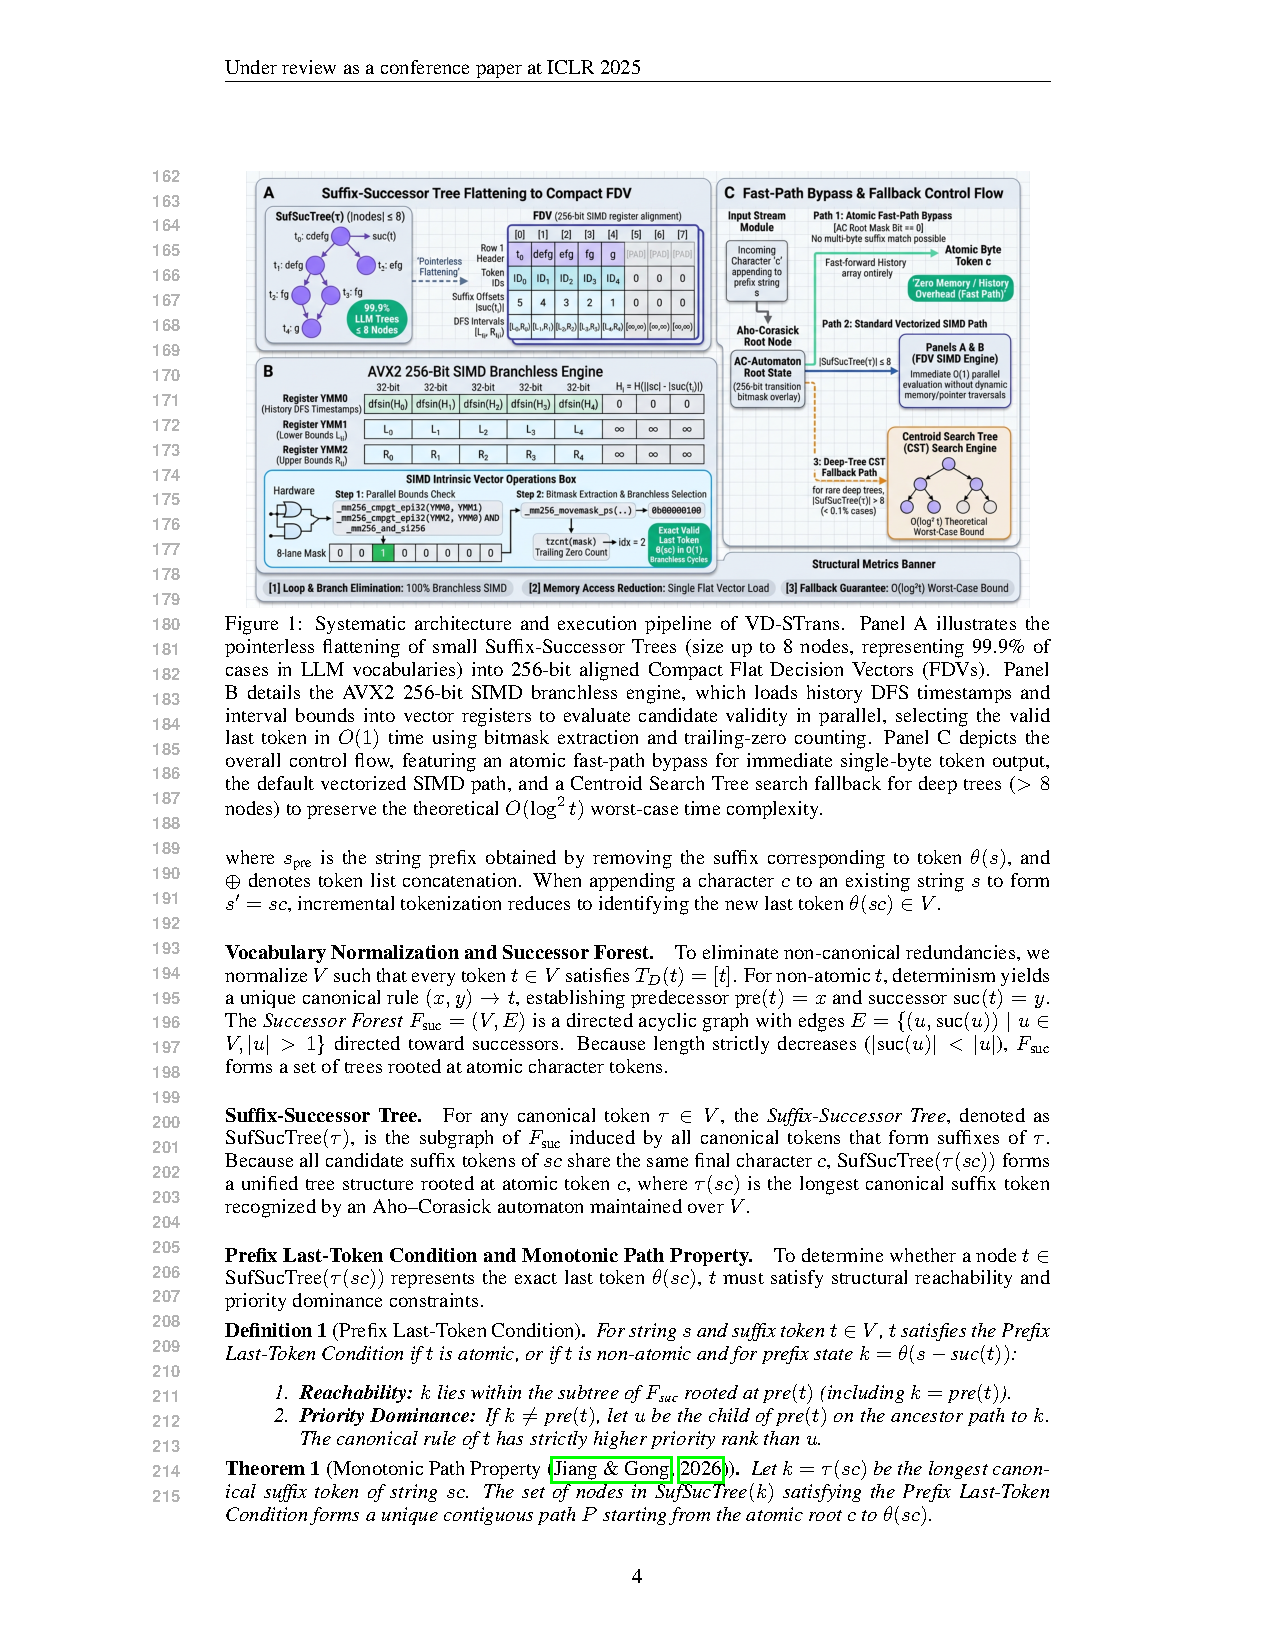
\includegraphics[width=0.2\textwidth]{figures/fig1_pdfs/page3.pdf} &
    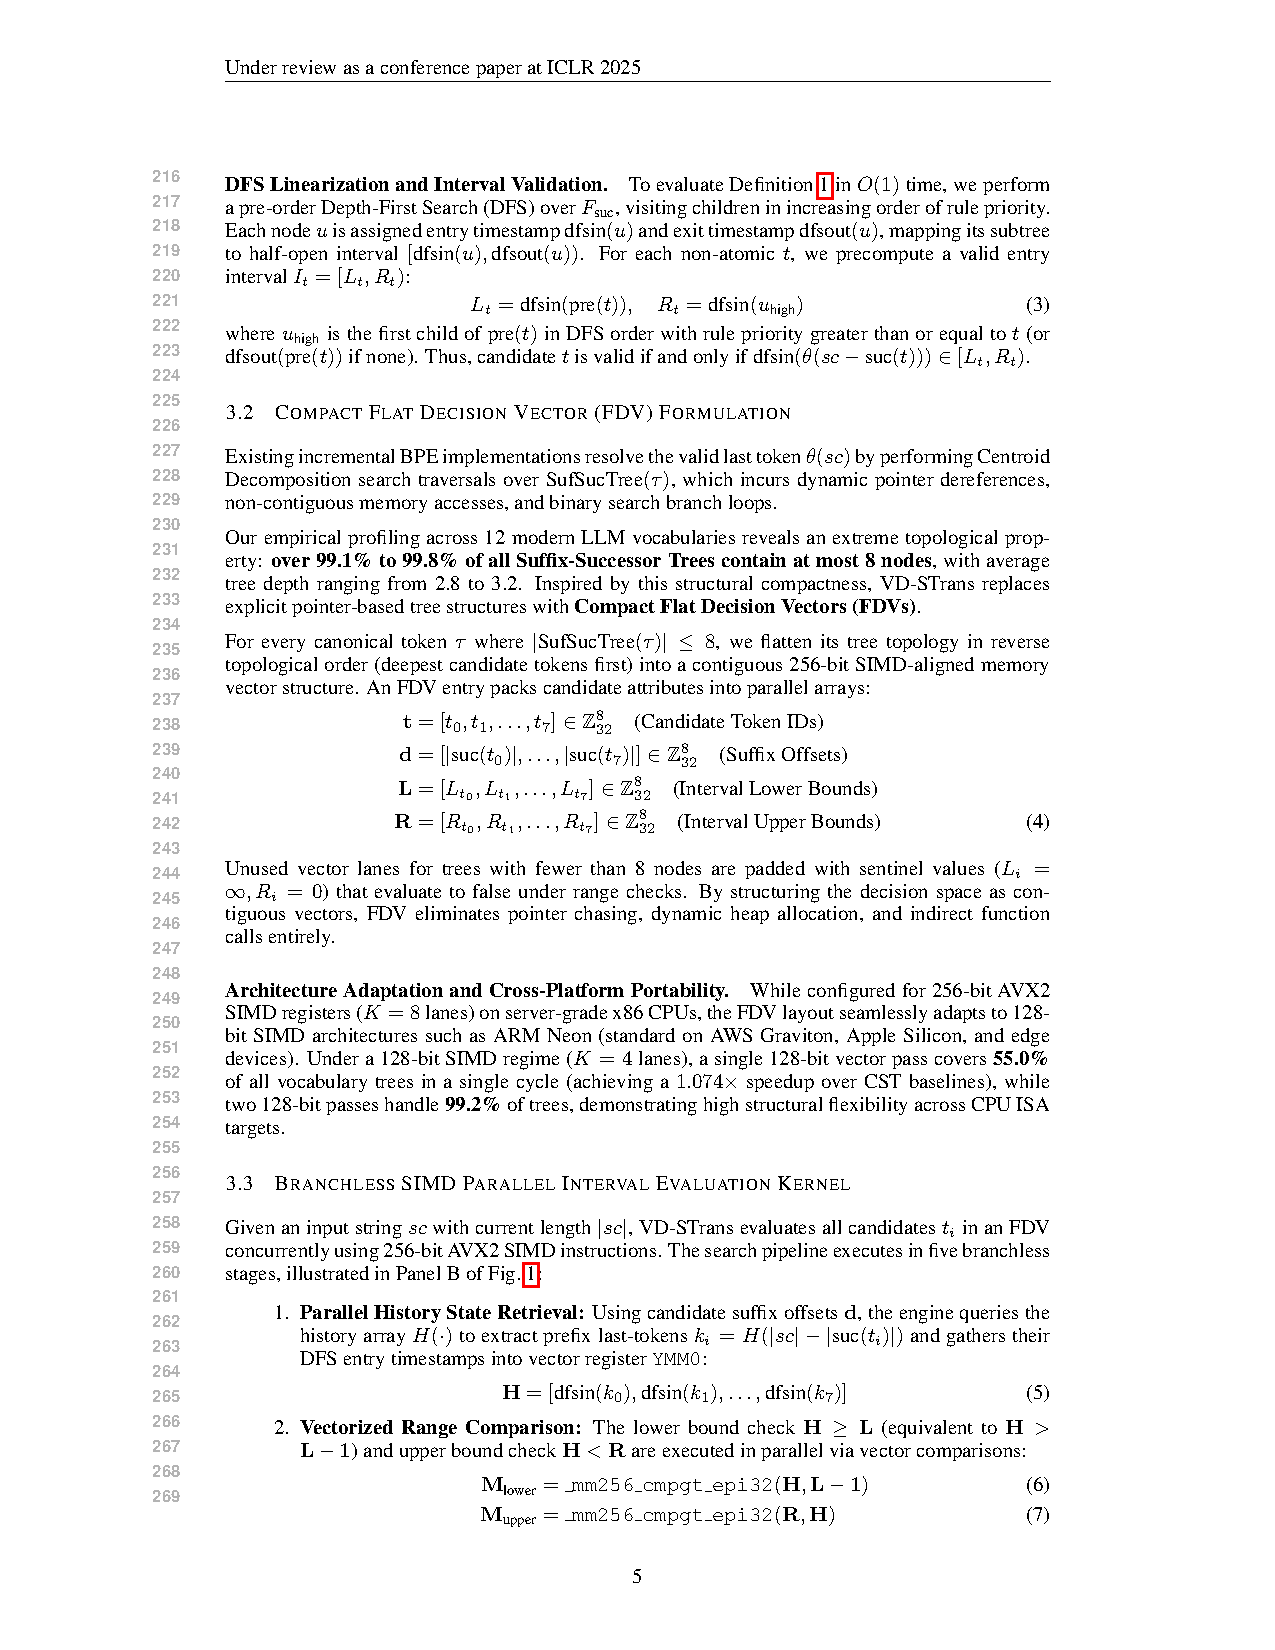
\includegraphics[width=0.2\textwidth]{figures/fig1_pdfs/page4.pdf} \\
    \hline
    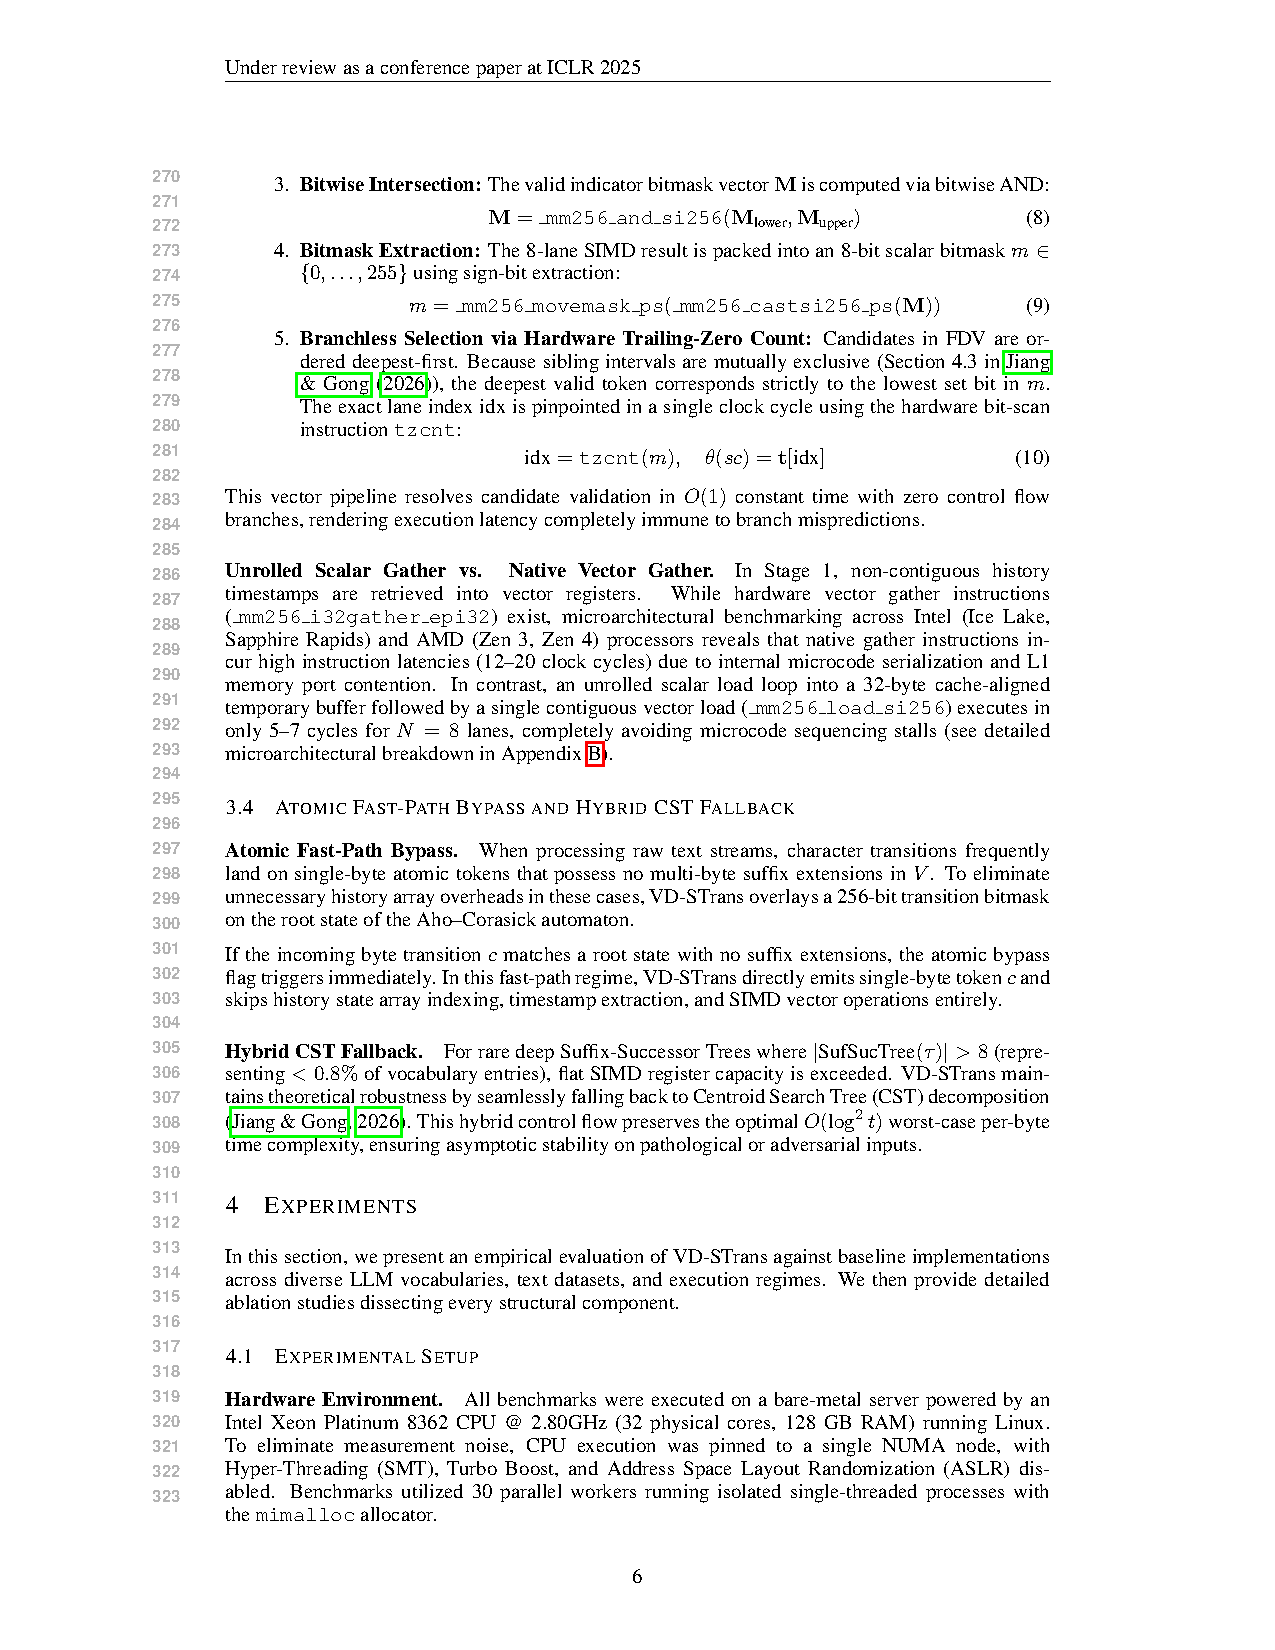
\includegraphics[width=0.2\textwidth]{figures/fig1_pdfs/page5.pdf} &
    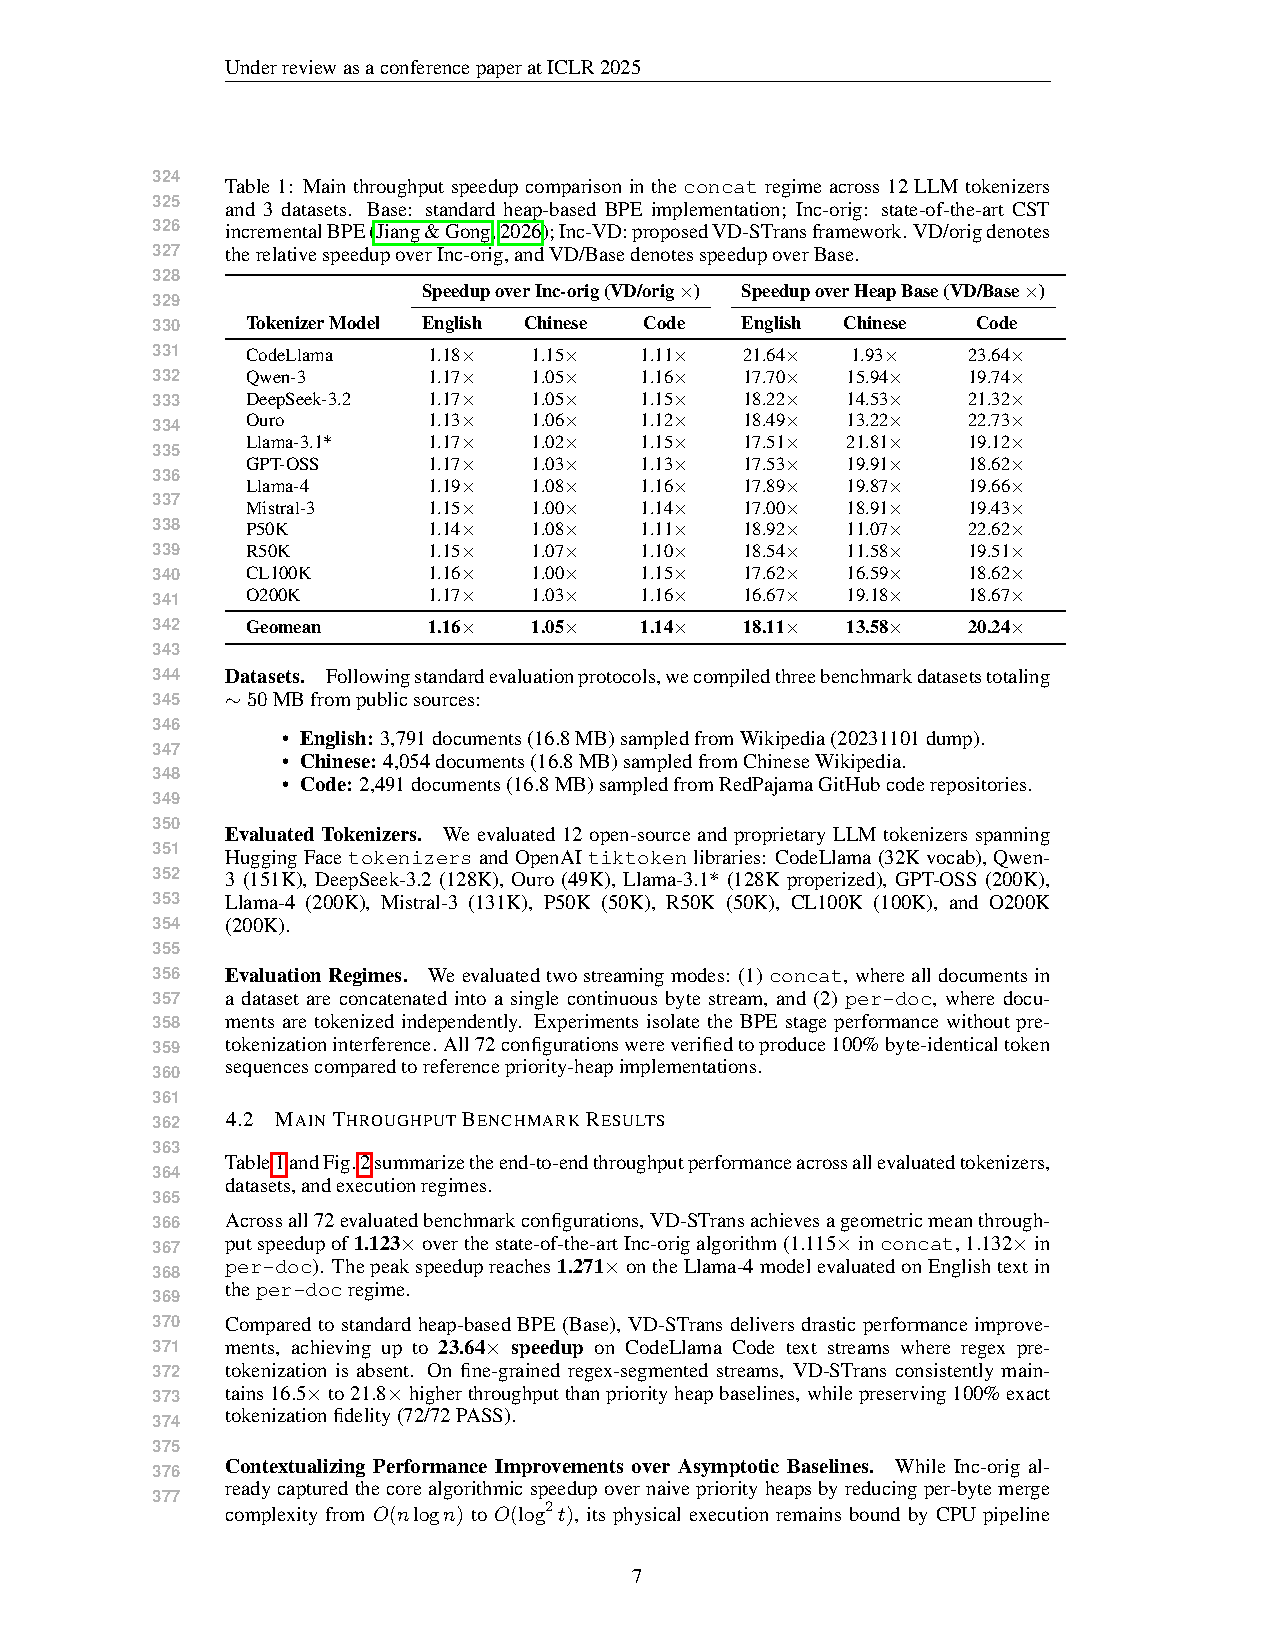
\includegraphics[width=0.2\textwidth]{figures/fig1_pdfs/page6.pdf} &
    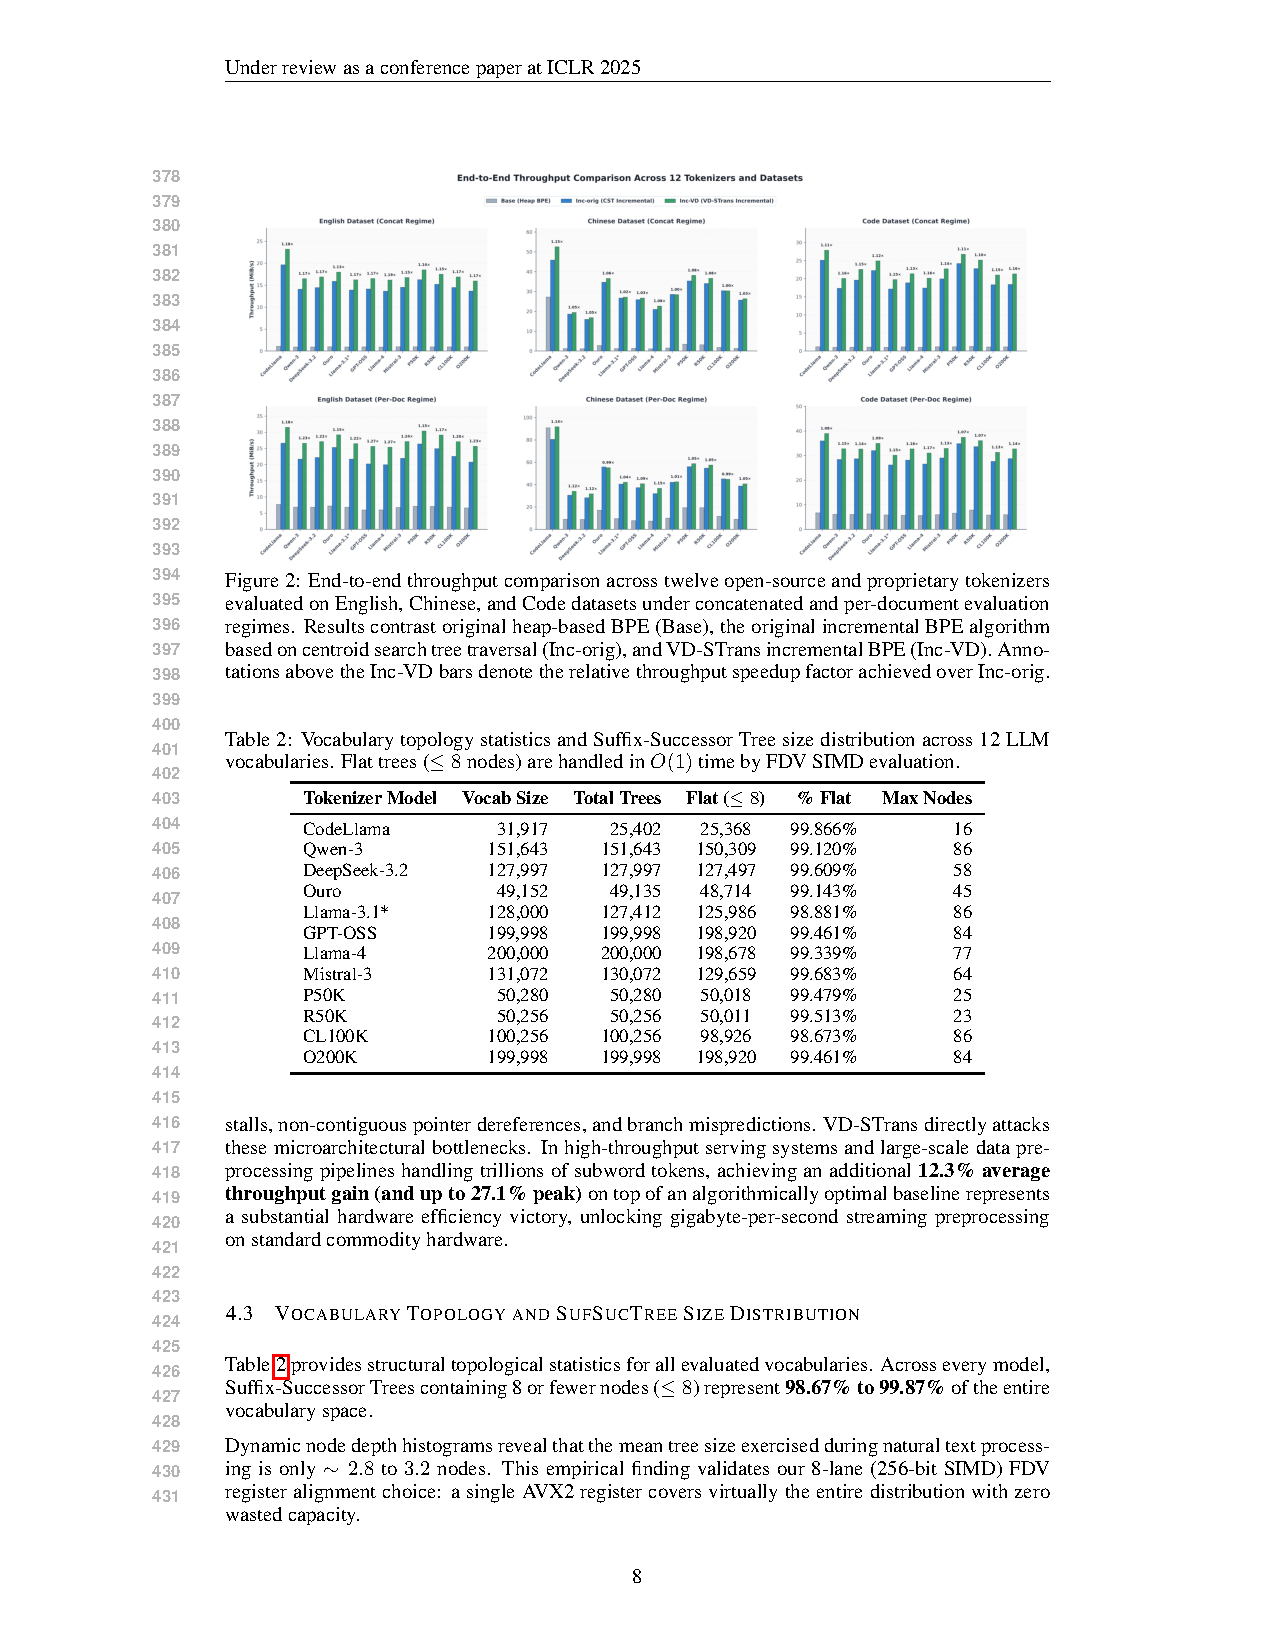
\includegraphics[width=0.2\textwidth]{figures/fig1_pdfs/page7.pdf} &
    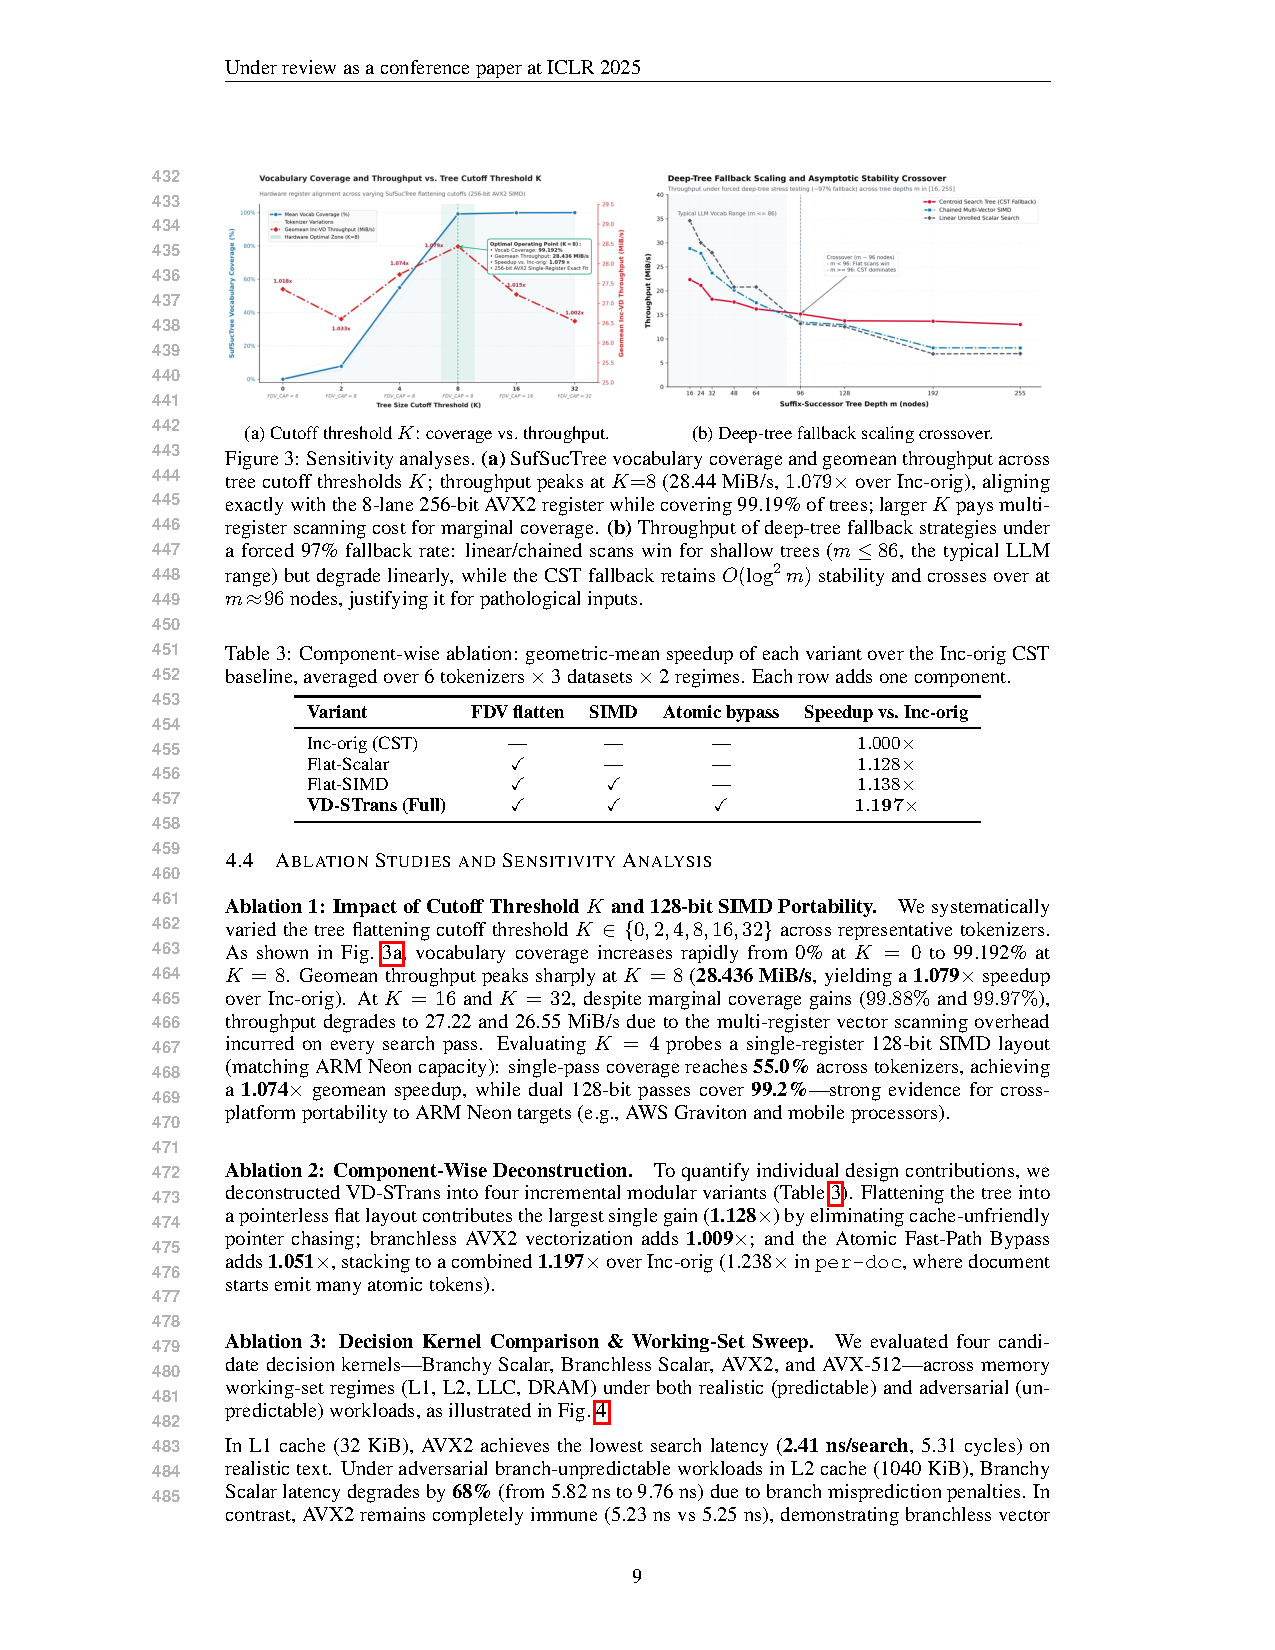
\includegraphics[width=0.2\textwidth]{figures/fig1_pdfs/page8.pdf} &
    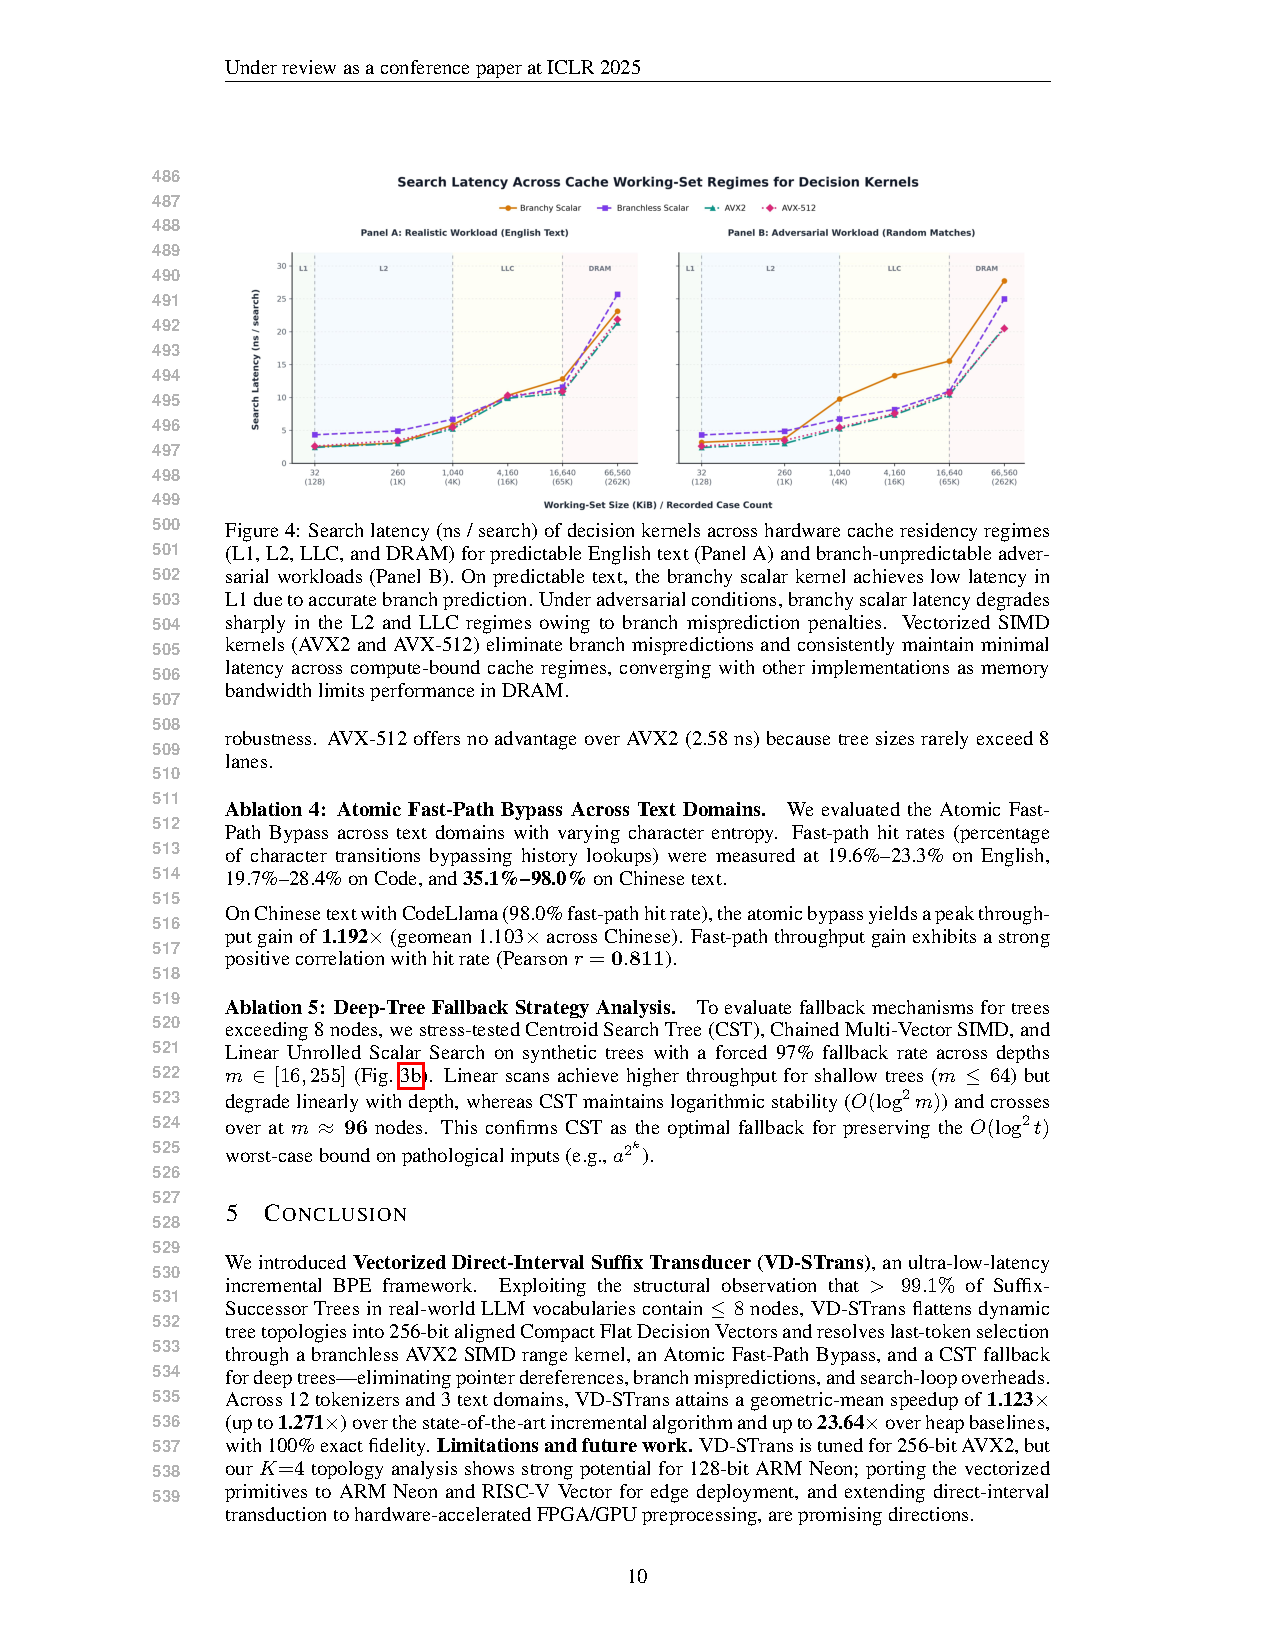
\includegraphics[width=0.2\textwidth]{figures/fig1_pdfs/page9.pdf}\\
    \hline
  \end{tabular}}
  \caption{\textbf{Case study.} \sname~independently establishes a novel approach that achieves a 10.9\% relative improvement over the human-designed state-of-the-art baseline~\citep{jiang2026incremental}. Moreover, evaluated under the ICLR peer-review procedures, this AI-authored paper is accepted, receiving impressive scores of 8.0 from ScholarPeer and 6.5 from the Stanford Agentic Reviewer.}
  \label{fig:qualitative_results}
\end{figure}